%% This paper describes the results of the Machine Learning practical
%% project. It should be approximately 8 pages long and contain the
%% following sections:
%%
%% 1) Title, authors, abstract
%% 2) Introduction
%% 3) Application
%% 4) Methods
%% 5) Experimental Results
%% 6) Discussion / Conclusion
%% References
\documentclass[preprint,journal,11pt]{vgtc}
\let\ifpdf\relax
%% Uncomment one of the lines above depending on where your paper is
%% in the conference process. ``review'' and ``widereview'' are for review
%% submission, ``preprint'' is for pre-publication, and the final version
%% doesn't use a specific qualifier. Further, ``electronic'' includes
%% hyperreferences for more convenient online viewing.

%% Please use one of the ``review'' options in combination with the
%% assigned online id (see below) ONLY if your paper uses a double blind
%% review process. Some conferences, like IEEE Vis and InfoVis, have NOT
%% in the past.

%% Please note that the use of figures is not permitted on the first page
%% of the journal version.  Figures should begin on the second page and be
%% in CMYK or Grey scale format, otherwise, colour shifting may occur
%% during the printing process.  Papers submitted with figures on the
%% first page will be refused.

%% These three lines bring in essential packages: ``mathptmx'' for Type 1
%% typefaces, ``graphicx'' for inclusion of EPS figures. and ``times''
%% for proper handling of the times font family.

\usepackage{mathptmx}
\usepackage{graphicx,xcolor,booktabs, tabularx,amsmath}
\usepackage{times}
\newcommand{\todo}[1]{\textbf{\textcolor{blue}{Todo: #1 }}}
%% We encourage the use of mathptmx for consistent usage of times font
%% throughout the proceedings. However, if you encounter conflicts
%% with other math-related packages, you may want to disable it.

%% If you are submitting a paper to a conference for review with a double
%% blind reviewing process, please replace the value ``0'' below with your
%% OnlineID. Otherwise, you may safely leave it at ``0''.
\onlineid{0}

%% declare the category of your paper, only shown in review mode
\vgtccategory{}

%% allow for this line if you want the electronic option to work properly
%\vgtcinsertpkg

%% In preprint mode you may define your own headline.
\preprinttext{}

%% Paper title.

\title{Comparing Machine Learning algorithms for classifying cognitive states from fMRI data}

%% This is how authors are specified in the journal style

%% indicate IEEE Member or Student Member in form indicated below
\author{Mattijs Meiboom, Robin Mills, Tijn Schouten, Spyros Ioakeimidis}
\authorfooter{
\item
  Mattijs Meiboom is with University of Groningen, E-mail: m.meiboom@student.rug.nl.
\item
  Robin Mills is with University of Groningen, E-mail: r.mills@student.rug.nl.
\item
  Tijn Schouten is with University of Groningen, E-mail: t.m.schouten.2@student.rug.nl.
\item
  Spyros Ioakeimidis  is with University of Groningen, E-mail: s.ioakeimidis@studenr.rug.nl.
}



%other entries to be set up for journal
%\shortauthortitle{}


%% Abstract section.
\abstract{
Functional magnetic resonance imaging (fMRI) is a brain mapping technique that allows researchers to infer activity in a subject's brain. This technique is typically used to determine which areas of the brain are involved in performing a certain task. Using this knowledge, we may also be able to determine what task was performed by looking at fMRI data. In this paper, we present a comparison of the performance of machine learning algorithms in between-subjects classification of cognitive states, using fMRI data. We found that averaging across ROIs gave the best classification performance. All classifiers that we used performed above-chance, and we found that a Multivariate Gaussian classifier outperformed a Naive Bayesian classifier and a Support Vector Machine. Overall we can say that machine learning algorithms provide a feasible method for decoding cognitive states from fMRI data.
} % end of abstract

%% Keywords that describe your work. Will show as 'Index Terms' in journal
%% please capitalize first letter and insert punctuation after last keyword
\keywords{fMRI, Machine learning, Classification.}

%% Copyright space is enabled by default as required by guidelines.
%% It is disabled by the 'review' option or via the following command:
\nocopyrightspace


\begin{document}

%% The ``\maketitle'' command must be the first command after the
%% ``\begin{document}'' command. It prepares and prints the title block.
%% the only exception to this rule is the \firstsection command
\firstsection{Introduction}
\label{sec:introduction}
\maketitle
%% Now the actual contents of first section
Human functional brain mapping is a field of study that has grown strongly in the past decades. This is not a surprise, because it is one of the few ways to look at brain activity of a living animal. There are several techniques available to scan for brain activity in a living human. Of these techniques, functional magnetic resonance imaging (fMRI) has become more and more popular because it has a very good spatial resolution (contrary to MEG/EEG), and it is non-invasive (contrary to PET). Brain activity is inferred from differences in the ratio between oxygenated and deoxygenated blood; when brain activity occurs, more oxygenated blood will flow to a brain region, and this change is detected by a machine. This is called the blood oxygen level dependent (BOLD) response \cite{sm:2012fMRI}.

The fMRI scanner measures the activity in three-dimensional pixels called voxels, which are about 3 x 3 x 3 mm in size, and a brain scan is made somewhere between every 500ms and every few seconds. Before analysing the acquired data, it is usually pre-processed to account for head movements by participants in the scanner and to make between-subjects comparisons possible \cite{sl:2009rl}.

Traditionally, data from each voxel, or from a group of voxels, are analysed with analysis of variance. Voxels are usually convoluted with a haemodynamic response function in an attempt to infer the spiking neural activity from the slowly building and dropping BOLD response \cite{he:2002na} (see Figure~\ref{fig:bold_response}). In this setup, experimental conditions are the independent variables and a general linear model is fitted to each voxel, or group of voxels. By using this technique, voxels or brain areas can be identified that differ in their average BOLD response across conditions.\\
\begin{figure}
	\centering
	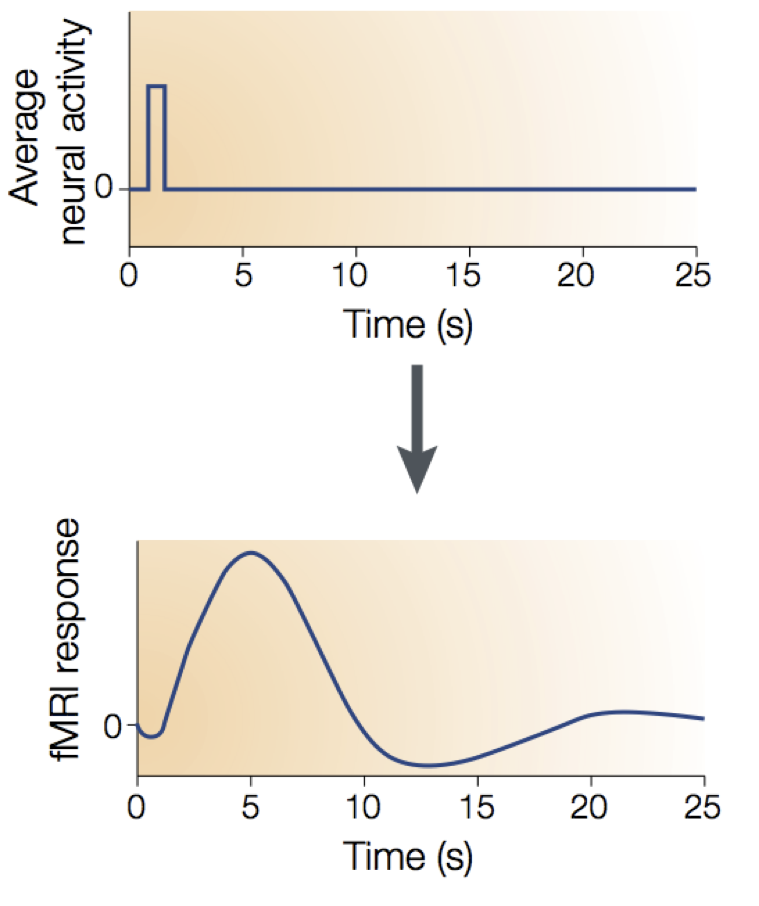
\includegraphics[width=60mm]{figures/f1_bold_response}
  	\caption{Above is the hypothetical neural response to some stimulus. Below is the BOLD response that is evoked by the short spike of neural activity. The neural activity shown above is attempted to be inferred from the BOLD response below that is measured by the fMRI scanner. Figure is adopted from Heeger and Ress \cite{he:2002na}.}
  	\label{fig:bold_response}
\end{figure}
\indent Recent studies indicate that this approach may have some serious limitations. One study used a dataset of 1326 subjects, which is much higher than the usual 15 to 25 subjects found in fMRI studies \cite{thy:2012very}. This study explored what happened to a simple contrast between BOLD signal while watching faces and baseline activity, when increasing the number of subjects included in the analysis. They found that, as the number of analysed subjects increased, an increasing number of brain areas that extended well beyond the expected visual- and face recognition areas showed significant deviation from baseline. Another study, using only three subjects, repeated a simple letter/number discrimination task and visual stimulation. The notable part is that this very simple experiment was run 100 times for each subject, again resulting in exceptionally high signal-to-noise ratio compared to conventional fMRI experiments. In this study the authors again found widespread significant BOLD-responses \cite{go:2012whole}. These findings suggest that significant deviations from baseline activity do not necessarily indicate any special involvement in the performed task, because almost the entire brain will show significant deviations given a high enough signal-to-noise ratio. These findings are perhaps not surprising, because everything we know about the brain indicates that it is best seen as a network with countless connections to other parts of the brain. Therefore, it makes sense to also analyse signals from the brain as a pattern of information coming from the entire brain, rather than attempting to link specific brain areas to experimental conditions.\\
\indent In fact, Machine learning algorithms have been employed in studies to learn the patterns of activity associated with some experimental condition. Subsequently, these learned patterns can be used on unseen subjects in order to predict experimental conditions from their brain activity patterns. If these predictions are accurate then it means that the identified patterns hold information about the brain activity associated with some experimental task.\\
\indent The general goal of these machine learning studies is to identify what experimental condition a subject is in at a certain time. The state that a person is in during some trial (e.g., looking at a face) is referred to as \emph{cognitive state}, because the cognitive processes that are associated with being in that state are of interest. Specifically, the aforementioned studies try to infer the cognitive state of a subject from the brain activity that is evoked in a subject by performing that trial. For example, in an experiment where subjects look at a set of pictures (e.g., a star and a plus), they would be in a certain cognitive state that is the result of looking at these pictures. One could then attempt to use machine learning on the fMRI signal that is evoked by the the brain activity associated with these cognitive states, and use this to learn what patterns of activity in the brain are associated with that cognitive state. This \emph{StarPlus} experiment has been performed by researchers where, in addition to viewing pictures, subjects also were tasked to read sentences containing some true or false statement about the pictures. These data have then been used to successfully infer the cognitive states of looking at either sentences or pictures within single subjects \cite{mi:2003within}, and between subjects \cite{wa:2003betw}.\\
\indent In this study we use the same StarPlus data as in the aforementioned experiment, and use machine learning algorithms to decode the cognitive states of subjects while looking at pictures or while looking at sentences. An interesting difference between many applications of machine learning, and this study is that most machine learning algorithms have the goal of achieving the maximum possible discrimination between conditions or classes. However, for fMRI studies it is important that the pattern of activity that is identified by the algorithm is a pattern associated with the cognitive state. When using non-linear classifiers, it is possible to decode features predictive of the cognitive state, where the brain does not actually respond to these features. For example, when decoding the primary visual cortex with high enough spatial resolution, it would be possible to combine simple features with a non-linear neural network to decode the presence or absence of, for example, faces. However, this information is not actually processed in that part of the brain \cite{to:2012rev}. To avoid this problem it is recommended to only use linear classifiers when decoding cognitive states from fMRI data. The classifiers that we compare in this paper are a Gaussian Naive Bayesian (GNB) classifier, Linear Support Vector Machine (LSVM), and a Multivariate Gaussian (MVG) classifier.\\
\indent The goal of this study is to compare the classification performance of the cognitive states associated with looking at a picture or looking at a sentence between subjects. This objective introduces an important issue, namely, how the data from the fMRI scans can be compared between subjects. There are two main ways this could be achieved. First, groups of voxels that are anatomically defined as belonging to a certain brain region, a so-called region of interest (ROI), can be averaged into a single \emph{supervoxel}, which can be compared between subjects. Second, a talairach coordinate system can be used that maps the voxels of each subject onto an anatomically defined coordinate. The ROI averaging it is a rather crude method, and a lot of information of the individual voxels is lost. However, because the ROIs are relatively easy to identify by an expert they can be compared easily between subjects. By using the Talairach coordinate system the data of each individual voxel can be used~\cite{talairach1988co}. However, because the error of doing this is usually in the order of a centimetre, while the size of the voxels are in the order of millimetres, the coordinates are difficult to generalise. Because we aim to do between-subjects comparisons the generalisation performance is important, thus we will use averaged ROIs in order to compare the classifiers \cite{mi:2004coord}.


%In the rest of this paper, we will discuss a number of machine learning techniques and their ability to classify our test data. In section~\ref{sec:methods} we will discuss the setup of our experiments and the analysis performed on our data. After that, in sections~\ref{sec:results} and ~\ref{sec:discussion}, we will present the results from these experiments and discuss them. We conclude this paper with a discussion on possible improvements and suggest some additional experiments that could be done.


\section{Application}
\label{sec:application}
Thus far, machine learning techniques have been successfully applied for decoding the orientation of a stimulus from fMRI scans \cite{ka:2005decoding}, identifying different patterns of activity for animate versus inanimate objects \cite{kr:2008RSA}, and even reconstructing visual input based on information in the fMRI scans \cite{mi:2008re}. The reason that these machine learning techniques work so well is that patterns of voxel activity can be identified rather than a significant deviation from some baseline. Specifically, information can be present in the pattern of voxels that belong to a certain brain region, even when the average signal from that region is zero (i.e., on average it does not differ from the baseline condition) \cite{to:2012rev}.

The studies mentioned before all depend on the question of whether fMRI data carry class
information (pattern discrimination) and exploiting this information to perform classification. However, researchers have indicated at least two other basic questions to which classifiers can be applied, being ``where or when
is class information represented?'' (pattern localization) and ``how is
class information encoded'' or ``how does its encoding relate to known
relationships between stimuli'' (pattern characterization)~\cite{pereira2009machine}. While the main focus of this paper is on the application of machine learning techniques in pattern discrimination, we will briefly discuss these two other applications.


\section{Methods}
\label{sec:methods}
The general approach for applying machine learning techniques to fMRI data consists of the following steps:
\begin{enumerate}
  \item Preprocessing
  \item Dimensionality reduction
  \item Training
  \item Testing
\end{enumerate}
The choices made in each of the steps affect the classifier accuracy. For a complete picture of the classification accuracies, we therefore try several methods at each step. In the following sections, these methods will be described.


- analysis / tools (python etc)

\subsection{Data Acquisition and Dimensions}
The dataset used for our experiments was originally collected by Marcel Just et al. from Carnegie Mellon University's Center for Cognitive Brain Imaging and published as the StarPlus fMRI dataset. This set consists of fMRI data for 6 subjects that was obtained while having each subject participate in a number of trials.

In some of these trials (baseline trials), no stimulus was presented and participants were instructed to remain inert. In other trials, subjects were presented with a sequence of two stimuli on a computer screen. The first stimulus was either a picture or a sentence lasting 4 seconds, followed by a blank screen of 4 seconds. After the blank screen, the opposite type of stimulus was presented for 4 seconds, followed by a blank screen of 15 seconds, during which the subject would indicate by pressing a button whether the sentence correctly described the picture. During each trial, approximately 54 fMRI scans have been taken with an interval of 500ms. In total, 14 trials were baseline trials, while half of the remaining trials had a picture as first stimulus and the other half a sentence.  
The entire dataset consists of voxel data and meta-data providing information about the dataset. Included in this information is not only the trial and scan each voxel belongs to, but also the type of the trial (picture first or sentence first). This makes the dataset suitable for classification using supervised learning.

In total, we have data available for approximately 4800 voxels per scan, 54 scans per trial, 40 trials per subject (excluding baseline trials) and 6 subjects. Voxels have been grouped into 25 ROIs (see \textit{Feature selection}).

Here we will need a nice picture, perhaps a pagewide one with labels of data for 1 trial?

\subsection{Preprocessing}

\subsection{Dimensionality Reduction}
\label{sec:dimensionalityReduction}
%Useful background info: http://www.brainvoyager.com/bvqx/doc/UsersGuide/WebHelp/Content/MVPATools/MVPA_Basic_Concepts.htm
Typical input for the machine learning algorithms discussed in this paper consists of a number of feature vectors, one for each fMRI scan. Such a feature vector $\vec{x}$ contains measures for the $N$ features we use to represent that scan and is derived from our input data. In the most basic case, we could use the entire set of voxels belonging to a scan, resulting in a feature vector containing potentially (hundreds of) thousands of features.
In the case that we have a very large dimension of features combined with only a limited amount of scans, our classifier may have difficulty learning the right classification function. This problem is formally known as the \textit{Hughes effect}\cite{Hughes1054102} which states that the predictive power of a machine learning algorithm decreases as the dimensionality increases with a fixed number of training examples. To reduce the dimensionality of the input, several different methods were used.

\emph{ROI mapping.} ROI mapping is a form of feature selection, wherein only a subset of the N-dimensional input space is used. As described in the introduction, ROIs are anatomically defined brain areas classified as relevant by an expert in the field. We used 7 of the 25 defined ROIs, labeled  'CALC' 'LIPL' 'LT' 'LTRIA' 'LOPER' 'LIPS' and  'LDLPFC'. These ROIs have previously been found to be most relevant in discriminating between the cognitive states of looking at sentences or pictures \cite{wa:2003betw}. To further reduce the number of features, average voxel values within these regions are taken as new input features. As other higher-order features such as the standard deviation, kurtosis and skewness within ROIs did not increase predictability, these were not included in the subsequent analysis. The disadvantage of using ROIs is that they require \textit{a priori} knowledge. When this knowledge is inaccurate, classification accuracy may not be optimal.

\emph{Principal Component Analysis (PCA).} As feature extraction method, we applied PCA. Ideally, the input vectors of the PCA should be the standardized Talairach coordinates, because we are conducting between-subject classification. As this coordinate system appeared to be inaccurate for this dataset, we were forced to use the voxel indices. The problem is that indices of different subjects may not map well onto each other, due to differences in brain size and shape. As a result, the accuracy of the PCA may be greatly reduced.   

\emph{Temporal dimensionality reduction.} The BOLD response peaks at approximately 5 seconds after a stimulus is presented (see Fig. 1). This means that the first scans after a stimulus may not represent activity related to this stimulus and should not be used for classification. To examine which scans provide maximal class information, we plotted the average BOLD activity per scan for all trials of all subjects, given a trial type and ROI. As can be seen in Figure~\ref{fig:boldroi}, scans 10 to 20 provide maximal information for the first stimulus, while scans 23 to 33 provide maximal information for the second stimulus. The other scans were excluded.      
\begin{figure}
	\centering
	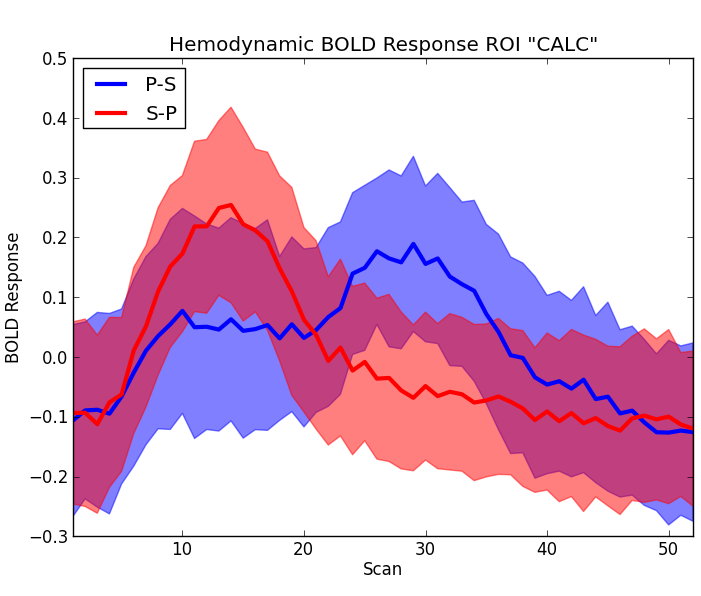
\includegraphics[width=90mm]{figures/scan_hemodynamic_BOLD_roi}
  	\caption{Haemodynamic BOLD response for ROI "CALC". The red line depicts a sentence-picture trial (S-P) and the blue line depicts a picture-sentence trial (P-S). Average Bold activity for all subjects is plotted against the scan number. The coloured regions depict an interval of 1 standard deviation.}
  	\label{fig:boldroi}
\end{figure}

\subsection{Training Method and Classifiers}
For each classifier, a "leave one (subject) out" cross validation procedure was used to avoid overfitting. For N=6 iterations, N-1 subjects functioned as training set, while the remaining subject served as validation set. The classifier accuracy is the average accuracy over all iterations. 
We compared the following classifiers:

\emph{Gaussian Naive Bayes (GNB).} This classifier builds a generative model underlying a class, by estimating the means and the standard deviations of the input features from the training set \cite{bk:2004aplay}. It assumes a Gaussian distribution and independent input features. Bayes rule is used to estimate the probability of a class (picture or sentence), given the input features of the validation set. Two approaches were used to estimate the parameters of the model. In the first method, averages of the selected scans belonging to a stimulus were used to estimate the parameters, while in the second method, the parameters were estimated for each scan. In both methods, the resulting probability of a class was the sum of log-likelihoods per scan and the class with maximum probability was selected. The advantage of the first method is that fewer parameters need to be estimated with greater amount of examples. It thus reduces the space and time complexity, and variance of the model. However, because it is likely that the assumptions of equal means and standard deviations for each scan do not hold, the second approach may decrease the inductive bias and enhance the accuracy.  

Linear Support Vector Machine.

Multivariate Gaussian (MVG). In MVG, independence between feature vectors is not assumed. Instead, the mutivariate distribution is used to estimate the probability of the classes, with the covariance matrix and the means as parameters. Again, the increase in parameters to be estimated compared to GNB (the correlations) may decrease generality, while also decreasing inductive bias.


- same for each algorithm:
    - What features did we select?
    - How did we train?
    - How did we test?
        - How did we calculate performance?
- algorithms:
    - gaussian naive-bayes (gnb)
        - pca + gnb
    - multivariate
    - svm
    - why multivariate is not a priori better than naive: less assumption, higher generalizability, better estimation parameters. 



\section{Experimental Results}
\label{sec:results}

\begin{table*}[htpb]
\centering
{\small
\begin{tabular}{c|c|c|c|c}
& \textbf{Naive Bayes} & \textbf{Linear SVM} & \textbf{Naive Bayes*} & \textbf{Multivariate*} \\ \hline
PCA & 61.46 &  - & - & - \\
M ROIs & 70.21 & 72.5 & 74.79 & 76.67 \\
Norm-M ROIs & 71.67 & 71.25 & 75.83 & 77.08 \\
Norm-M-SD ROIs & 65.63 & 69.79 & 69.38 & 65.0 \\
Norm/Vox-M ROIs & 73.13 & 76.67 & 76.88 & 79.58 \\
\end{tabular}}
\caption{Performance results (in \%) of the three classifiers on different methods for feature selection and structure. \emph{M} stands for \emph{Mean}, \emph{Norm} for \emph{Normalisation}, \emph{SD} for \emph{Standard Deviation}, and \emph{Norm/Vox} for \emph{Normalisation per Voxel index}.}
\label{tab:results}
\end{table*}

As a comparison measure, we used the performance of the classifiers for predicting the cognitive state that a subject was in. The predictive performance of Naive Bayes, Linear SVM, and Multivariate was compared. We observed that different feature selection and extraction methods, as well as different structure on the data affects the predictive performance of the classifiers.

Table~\ref{tab:results} illustrates the overall performance of the three classifiers. Rows indicate various feature selection methods. We applied PCA to the original data, while the other classifiers were applied to the data belonging to the selected ROIs (cf.~Section~\ref{sec:dimensionalityReduction}). For instance, \emph{Norm/Vox-M-SD ROIs} indicates that we normalised over the voxel values of the same voxel index using the mean and standard deviation, while \emph{Norm-M-SD ROIs} indicates that we normalised over the voxel values of the same scan index using the mean and standard deviation. Columns depict the used classifiers. For the classifiers depicted with *, we used different structure for the data, as described in Section~\ref{}.

Furthermore, to test the significance of the differences in performance between the different methods we performed an exact binomial test in each case, from which we obtained the confidence interval. The results were rounded to one decimal point. For the following comparison we are only looking at the case where \emph{Norm/Vox-M-SD ROIs} was used.

From Table~\ref{tab:results} we can distinguish the fact that when PCA is used for feature extraction, the performance of Naive Bayes is lower than when other feature selection methods are used. The confidence interval of the predictive performance of Naive Bayes when PCA is used is 95\% $CI: 56.9 - 65.8$ which suggests that...

Comparing classifiers when the same data structure is used, we can distinguish the fact that Multivariate performs better than Naive Bayes. Also that Linear SVM performs better than Naive Bayes, though not significantly. The confidence interval of Naive Bayes is 95\% $CI: 68.9-77.0$ and of Linear SVM is 95\% $CI: 72.6-80.4$, which suggests that their performances do not differ significantly.

Moreover, when different data structure is used the performance increases, though not significantly. This can be seen by comparing the performance of Naive Bayes when different data structure is used. In the first case it is 73.13\% while in the second case is 76.88\%. The confidence interval in the first case is 95\% $CI: 68.9 - 77.0$ and in the second case is 95\% $CI: 72.8 - 80.6$.

Finally, we can distinguish the fact that Multivariate outperforms all the other classifiers, though we did not try a different data structure in the case of Linear SVM. However, we still do not expect that the performance of Linear SVM will be higher that this of Multivariate. The confidence interval of Multivariate is 95\% $CI: 75.7-83.1$.

\section{Discussion / Conclusion}
\label{sec:discussion}

In this paper we have replicated earlier findings of decoding the cognitive states of looking at sentences or pictures from fMRI data. Specifically, by observing the patterns of activity for a group of subjects, we are able to predict with above-chance accuracy what the cognitive state of an unseen subject is. This shows that machine learning algorithms can be employed to capture useful information from noisy data, and generalise this information between subjects.\\
\indent We found that even though all of our classification procedures yielded well above chance-level classification performance, the differences between the classifiers was very seldom significant. Still, we consistently found that the Multivariate Gaussian (MVG) classifier outperformed the Gaussian Naive Bayes (GNB) classifier and Linear Support Vector machine (LSV). This finding suggests that the interactions between different brain areas contain information about the cognitive state, and that these functional connectivity generalises to an extent to different subjects.\\
\indent Still, the uncertainty in our predictions are relatively high, with maximum classification performance reaching close to 80\% accuracy for only two classes. The noisy nature of the fMRI data therefore makes it very difficult to draw hard conclusions when decoding a single cognitive state from a brain scan. This is something to be considered before employing fMRI as a diagnostic tool, or as evidence in court.\\
\indent Overall we can say that machine learning provides a feasible way of extracting useful information from fMRI data. Furthermore, it avoids a strict multiple comparisons correction that is required in null hypothesis testing by using cross-validation. Also, the identification of patterns of activity associated with tasks is encouraged, rather than attempting to identifying brain regions that are involved in tasks. In doing this, much can be learned about how information is represented and processed in the brain.


\bibliographystyle{abbrv}
%%use following if all content of bibtex file should be shown
%\nocite{*}
\bibliography{references}
\end{document}